\documentclass[../main.tex]{subfiles}
\LoadClass[a4paper,12pt]{article}
\documentclass{article}

%%%%%%%%%%%%%%%%%%%%%%%%%%%%%%%
%     import des packages     %
%%%%%%%%%%%%%%%%%%%%%%%%%%%%%%%
\usepackage[export]{adjustbox}
\usepackage{algorithm}
\usepackage{algorithmic}
\usepackage{amsmath,amsfonts,amssymb}
\usepackage{anyfontsize}
\usepackage{array}
\usepackage[english]{babel}
\usepackage{colortbl}
\usepackage{comment}
\usepackage{cclicenses}
\usepackage{eqnarray}
\usepackage{eso-pic}
\usepackage{dirtree}
\usepackage{fancybox}
\usepackage{fancyhdr}
\usepackage{float}
\usepackage[T1]{fontenc} 
\usepackage{forest}
\usepackage{fourier-orns}
\usepackage{gensymb}
\usepackage{geometry}
\usepackage{glossaries}
\usepackage{graphicx}
\usepackage{hyperref}
\usepackage{ifthen}
\usepackage{import}
\usepackage{indentfirst}
\usepackage[utf8]{inputenc}
\usepackage{lastpage}
\usepackage{libertine}
\usepackage{lipsum}
\usepackage{listings}
\usepackage{mathtools}
\usepackage{mdframed}
\usepackage{multicol}
\usepackage{pdfpages}
\usepackage{pifont}
\usepackage{stmaryrd}
\usepackage{subcaption}
\usepackage{subfiles}
\usepackage{tabularx}
% \usepackage{tcolorbox}
\usepackage[most]{tcolorbox}
\usepackage{textcomp}
\usepackage{ulem}
\usepackage{wrapfig}

%%%%%%%%%%%%%%%%%%%%%%%%%%%%%%%%%%%%%%%%%%%%%%%%%%%%%%%%%
%    Renseigner les titres et variables importantes     %
%%%%%%%%%%%%%%%%%%%%%%%%%%%%%%%%%%%%%%%%%%%%%%%%%%%%%%%%%
\newcommand{\titre}{Multi-robot coordination}
\newcommand{\soustitre}{Autonomous exploration of gallery networks}
\newcommand{\sujet}{Engineering Graduation Project}
\newcommand{\sujets}{Seatech 3A - MOCA}
\newcommand{\auteur}{Fabien MATHÉ}
\newcommand{\referent}{M. Mehmet ERSOY}
\newcommand{\reportdate}{\date}

\newcommand{\partA}{State of the art}
\newcommand{\partB}{Partie 2}
\newcommand{\partC}{Partie 3}
\newcommand{\partD}{Partie 4}
\newcommand{\partE}{Partie 5}

%%%%%%%%%%%%%%%%%%%
%     BOOLEEN     %
%%%%%%%%%%%%%%%%%%%

% Création des boolean
\newboolean{abst}
\newboolean{thx}
\newboolean{contents}
\newboolean{introduction}
\newboolean{pt2}
\newboolean{pt3}
\newboolean{pt4}
\newboolean{pt5}
\newboolean{conclusion}
\newboolean{perspectives}
\newboolean{glossaire}
\newboolean{biblio}
\newboolean{annexe}


% Renseigner si le Rapport contient un abstract
\setboolean{abst}{true}
% Renseigner si le Rapport contient des remerciements
\setboolean{thx}{true}
% Renseigner si le Rapport contient une table des matières
\setboolean{contents}{true}
% Renseigner si le Rapport contient une introduction
\setboolean{introduction}{true}
% Renseigner si le Rapport contient une partie 2
\setboolean{pt2}{true}
% Renseigner si le Rapport contient une partie 3
\setboolean{pt3}{true}
% Renseigner si le Rapport contient une partie 4
\setboolean{pt4}{true}
% Renseigner si le Rapport contient une partie 5
\setboolean{pt5}{true}
% Renseigner si le Rapport contient une introduction
\setboolean{conclusion}{true}
% Renseigner si le Rapport contient des perspectives
\setboolean{perspectives}{true}
% Renseigner si le document contient une bibliographie
\setboolean{biblio}{true} 
% Renseigner si le document contient un glossaire
\setboolean{glossaire}{false}
% Renseigner si le Rapport contient des annexes 
\setboolean{annexe}{true}


%%%%%%%%%%%%%%%%%%%%%%%%%%%%%%%%%%%%%%
%     En-têtes en pieds de pages     %
%%%%%%%%%%%%%%%%%%%%%%%%%%%%%%%%%%%%%%
\geometry{hmargin=2cm,vmargin=2.3cm}
\pagestyle{fancy}
\fancyhfoffset[]{0pt}
\setlength{\headheight}{28pt}
\lhead{
\includegraphics[height = 0.6cm]{IMAGES/logos/Logo_SeaTech_2023.png}}
% \rhead{
\includegraphics[height = 0.7cm]{IMAGES/logos/MOCA.png}}
\rhead{\textsc{\leftmark}}

% Update \rightmark with \section name
\renewcommand{\sectionmark}[1]{\markboth{#1}{#1}}


\lfoot{\auteur}
\cfoot{ }
\rfoot{Page \thepage \ / \pageref{LastPage}}

\title{\titre}
\author{\auteur}
\date{\today}

%%%%%%%%%%%%%%%%%%%%%%%%%%%%%%
%     Autre mise en page     %
%%%%%%%%%%%%%%%%%%%%%%%%%%%%%%
\numberwithin{figure}{section}
\numberwithin{table}{section}

\setcounter{tocdepth}{2} % Change to 1 to exclude subsections as well


\newcommand{\citeURL}[1]{\href{#1}{\detokenize{#1}}}

% Création du compteur d'annexes
\newcounter{annexecounter}

% Définition de la commande pour les annexes
\NewDocumentCommand{\annexe}{m}{%
    \stepcounter{annexecounter} % Incrémenter le compteur d'annexes
    \subsection*{Annexe \arabic{annexecounter} - #1} % Affichage du texte avec le numéro et le titre
	\label{sec:#1}
}

\newcommand{\tobedone}{\textcolor{red}{\LARGE \textbf{TO BE DONE}}}
\newcommand{\annexetonum}{\textcolor{red}{\LARGE \textbf{ANNEXE ...}}}

\renewcommand{\familydefault}{\sfdefault}



%%%%%%%%%%%%%%%%%%%%%%%%%%%%%%%%%
%     Mise en page des codes    %
%%%%%%%%%%%%%%%%%%%%%%%%%%%%%%%%%
\definecolor{codegreen}{rgb}{0,0.6,0}
\definecolor{codegray}{rgb}{0.5,0.5,0.5}
\definecolor{codepurple}{rgb}{0.58,0,0.82}
\definecolor{backcolour}{rgb}{0.95,0.95,0.92}

\lstdefinestyle{python}{
	backgroundcolor=\color{backcolour},
	commentstyle=\color{codegreen},
	keywordstyle=\color{blue},
	numberstyle=\tiny\color{codegray},
	stringstyle=\color{codepurple},
	basicstyle=\ttfamily\scriptsize,
	breakatwhitespace=false,
	breaklines=true,
	captionpos=b,
	keepspaces=true,
	numbers=left,
	numbersep=5pt,
	showspaces=false,
	showstringspaces=false,
	showtabs=false,
	tabsize=2
}

\lstset{style=python}
\definecolor{codegreen}{rgb}{0,0.6,0}
\definecolor{codegray}{rgb}{0.5,0.5,0.5}
\definecolor{codepurple}{rgb}{0.58,0,0.82}
\definecolor{backcolour}{rgb}{0.95,0.95,0.92}

\lstdefinestyle{cpp}{
	backgroundcolor=\color{backcolour},
	commentstyle=\color{codegreen},
	keywordstyle=\color{blue},
	numberstyle=\tiny\color{codegray},
	stringstyle=\color{codepurple},
	basicstyle=\ttfamily\scriptsize,
	breakatwhitespace=false,
	breaklines=true,
	captionpos=b,
	keepspaces=true,
	numbers=left,
	numbersep=5pt,
	showspaces=false,
	showstringspaces=false,
	showtabs=false,
	tabsize=2,
	language=C++
}

\lstset{style=cpp}

\definecolor{codegreen}{rgb}{0,0.6,0}
\definecolor{codegray}{rgb}{0.5,0.5,0.5}
\definecolor{codepurple}{rgb}{0.58,0,0.82}
\definecolor{backcolour}{rgb}{0.95,0.95,0.92}

\lstdefinestyle{fortran}{
    backgroundcolor=\color{backcolour},
    commentstyle=\color{codegreen},
    keywordstyle=\color{blue},
    numberstyle=\tiny\color{codegray},
    stringstyle=\color{codepurple},
    basicstyle=\ttfamily\scriptsize,
    breakatwhitespace=false,
    breaklines=true,
    captionpos=b,
    keepspaces=true,
    numbers=left,
    numbersep=5pt,
    showspaces=false,
    showstringspaces=false,
    showtabs=false,
    tabsize=2,
    language=[90]Fortran
}

\lstset{style=fortran}


%%%%%%%%%%%%%%%%%%%%%%%%%%%%%%%%%%%%%%%%%%%%%%%%%%%%%%%%%%%%%%%%%%%%%%%%%%%%%%%%%%%%%%%%%%%%%%%%%%%%%%%%%%%%%%%%%%%%%%%
%                                                  Début du document                                                  %
%%%%%%%%%%%%%%%%%%%%%%%%%%%%%%%%%%%%%%%%%%%%%%%%%%%%%%%%%%%%%%%%%%%%%%%%%%%%%%%%%%%%%%%%%%%%%%%%%%%%%%%%%%%%%%%%%%%%%%%

\begin{document}

%%%%%%%%%%%%%%%%%%%%%%%%%
%     Page de garde     %
%%%%%%%%%%%%%%%%%%%%%%%%%
\begin{titlepage}
	\AddToShipoutPictureBG*{
\includegraphics[width=\paperwidth,height=\paperheight]{IMAGES/PageDeGardeRapport.png}}
	\begin{figure}[H]
		\begin{subfigure}{0.45\linewidth}
				
\includegraphics[width=0.6\textwidth,left]{IMAGES/logos/Logo_SeaTech_2023.png}
		\end{subfigure}
		\hfill
		\begin{subfigure}{0.45\linewidth}
				% 
\includegraphics[width=0.6\textwidth,right]{IMAGES/logos/MOCA.png}
		\end{subfigure}
	\end{figure}

	\centering

	% Espacement vertical
	\vspace*{5cm}

	% Barres horizontales
	\makebox[0.7\linewidth]{\hrulefill}\\[0.2cm]

	% Titre encadré
	\vspace{0.5cm}
	\begin{minipage}{\textwidth}
		\centering
		{\fontsize{28}{48}\selectfont \textsc{\titre}}\\[0.2cm]

		{\fontsize{18}{48}\selectfont \textsc{\soustitre}}
	\end{minipage}
	\vspace{0.3cm}

	% Barres horizontales
	\makebox[0.8\linewidth]{\hrulefill}\\[0.2cm]

	% Espacement vertical
	\vspace{3cm}

	% Description
		\large{\Large \textbf{\sujet}}\\
		\large{\textbf{\sujets}}\\

		\vspace{0.5cm}
		\large{\textbf{\reportdate}}

	\vspace{2cm}

	\begin{minipage}{0.20\textwidth}

	\end{minipage}
	\hfill
	\begin{minipage}{0.35\textwidth}
		\begin{flushleft}
			Auteur : \\
			\auteur
		\end{flushleft}
	\end{minipage}
	\begin{minipage}{0.09\textwidth}
		% Section vide pour espacement optimal
	\end{minipage}
	\hfill
 	\begin{minipage}{0.3\textwidth}
		\begin{flushleft}
			Enseignant : \\
			\referent

		\end{flushleft}
	\end{minipage}


\end{titlepage}

\ClearShipoutPictureBG

\newpage

\renewcommand{\thepage}{}

\renewcommand{\thepage}{\arabic{page}}
\renewcommand{\thesection}{\Roman{section}}

%%%%%%%%%%%%%%%%%%
%     Résumé     %
%%%%%%%%%%%%%%%%%%
\ifthenelse{\boolean{abst}}{
	\addcontentsline{toc}{section}{\protect\numberline{}Résumé}%
	\subfile{SECTIONS/1resume}

	\newpage
}

%%%%%%%%%%%%%%%%%%%%%%%%%
%     Remerciements     %
%%%%%%%%%%%%%%%%%%%%%%%%%
\ifthenelse{\boolean{thx}}{
	\addcontentsline{toc}{section}{\protect\numberline{}Remerciements}%
	\subfile{SECTIONS/2remerciements}

	\newpage
}

%%%%%%%%%%%%%%%%%%%%%%%%%%%%
%     Plan du document     %
%%%%%%%%%%%%%%%%%%%%%%%%%%%%

\ifthenelse{\boolean{contents}}{
	\vfill
	\tableofcontents
	\vfill
	
	\newpage
}

%%%%%%%%%%%%%%%%%%%%%%%%
%     INTRODUCTION     %
%%%%%%%%%%%%%%%%%%%%%%%%
\ifthenelse{\boolean{introduction}}
{
	\addcontentsline{toc}{section}{\protect\numberline{}Introduction}%
	\section*{Introduction}

	\markboth{Introduction}{Introduction} % Manually update \rightmark for section*
	\subfile{SECTIONS/3introduction}


	\newpage
}


%%% PARTIE 1 %%%
\section{\partA}
\subfile{SECTIONS/part1}

%%% PARTIE 2 %%%
\newpage
\ifthenelse{\boolean{pt2}}
{
	\section{\partB}
	\subfile{SECTIONS/part2}
	
	\newpage
}
	
	
%%% PARTIE 3 %%%
\ifthenelse{\boolean{pt3}}
{
	\section{\partC}
	\subfile{SECTIONS/part3}
	
	\newpage
}
	
	
%%% PARTIE 4 %%%
\ifthenelse{\boolean{pt4}}
{
	\section{\partD}
	\subfile{SECTIONS/part4}
	
	\newpage
}
	
%%% PARTIE 5 %%%
\ifthenelse{\boolean{pt5}}{
	\section{\partE}
	\subfile{SECTIONS/part5}

	\newpage
}
		
%%%%%%%%%%%%%%%%%%%%%%
%     CONCLUSION     %
%%%%%%%%%%%%%%%%%%%%%%
\ifthenelse{\boolean{perspectives}}
{
	\addcontentsline{toc}{section}{\protect\numberline{}Conclusion}%
	\section*{Conclusion}
	\markboth{Introduction}{Introduction} % Manually update \rightmark for section*

	\subfile{SECTIONS/Wconclusion}

	\newpage
}



\ifthenelse{\boolean{perspectives}}
{
	\section*{Perspectives}
	\addcontentsline{toc}{section}{\protect\numberline{}Perspectives}
	\subfile{SECTIONS/Xperspectives}
	
	\newpage 
}

%%%%%%%%%%%%%%%%%%%%%%%%%
%     Bibliographie     %
%%%%%%%%%%%%%%%%%%%%%%%%%

\ifthenelse{\boolean{biblio}}
{
	\addcontentsline{toc}{section}{\protect\numberline{}References}
	% \bibliographystyle{unsrt}
	\bibliographystyle{IEEEtran}
	\footnotesize{\bibliography{BIBLIOGRAPHY/bib.bib}}

	\newpage
}


%%%%%%%%%%%%%%%%%%%%%
%     Glossaire     %
%%%%%%%%%%%%%%%%%%%%%
\normalsize
\ifthenelse{\boolean{glossaire}}
{
	\section*{Glossaire}
	\makeglossaries
	\printglossaries
	\addcontentsline{toc}{section}{\protect\numberline{}Glossaire}%
	\subfile{SECTIONS/Yglossaire}
	
	\newpage
}

%%%%%%%%%%%%%%%%%%%
%     Annexes     %
%%%%%%%%%%%%%%%%%%%
\ifthenelse{\boolean{annexe}}
{
	\section*{Annexes}
	\addcontentsline{toc}{section}{\protect\numberline{}Annexes}%
	\subfile{SECTIONS/Zannexes}
}


\end{document}


\begin{document}

\subsection{Purpose and range of the simulator}

The simulator is designed to test various algorithms and methods for multi-robot exploration of caves. The robots operate in the air while moving along the floor. To simplify the problem, we approximate the floor as a 2D plane without any surface irregularities.

\subsection{Creation of the map}

The map consist in succession of straight lines generate by a simple cellular automata. 

A cellular automaton is a grid of cells, where each cell can exist in different states based on predefined rules. The concept was developed by Stanislaw Ulam and John von Neumann in the 1940s.  

The most famous cellular automaton, which helped popularize its use, was developed by John Conway: \textit{Conway's Game of Life}. This model follows a set of four simple rules, which can be found \href{URL}{here}. The rules are based on the properties of neighboring cells.  

There are two commonly used neighborhood types in cellular automata:  
\begin{itemize}  
    \item \textbf{Von Neumann neighborhood}, which considers the four direct neighbors (left, top, right and bottom).  
    \item \textbf{Moore neighborhood}, an extension that includes all eight surrounding cells, both diagonal and direct neighbors.  
\end{itemize}


The beauty of this system lies in the complexity that emerges from such simple rules. Beginning with the configuration shown in \autoref{fig:startconfigcgof}, the system evolves into the states illustrated in \autoref{fig:CGOF} at generations 87 and 263.

\begin{figure}[H]
    \centering
    \begin{subfigure}{0.2\textwidth}
        \centering
        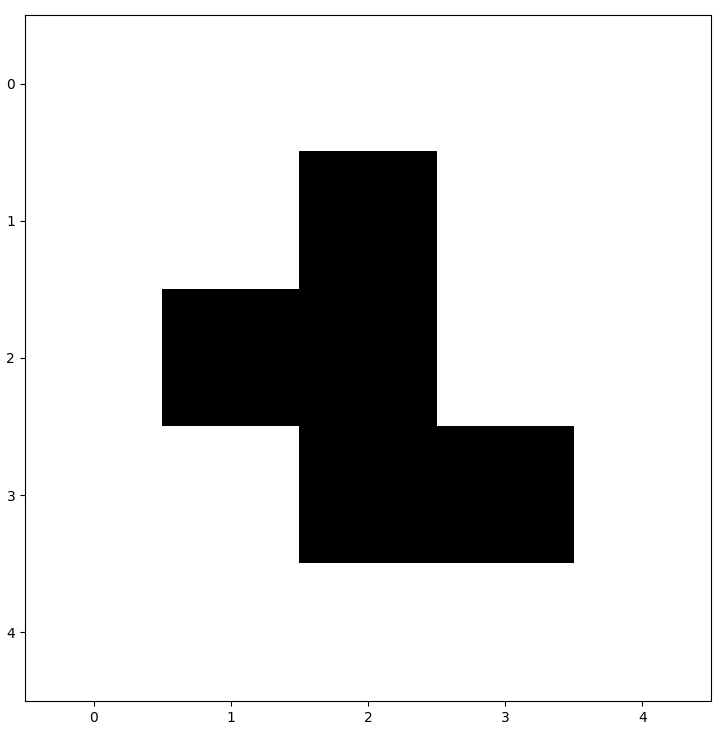
\includegraphics[width=\textwidth]{IMAGES/part2/StartConfigCGOF.png}
        \caption{Iteration 0}
		\label{fig:startconfigcgof}
    \end{subfigure}
    \hfill
    \begin{subfigure}{0.35\textwidth}
        \centering
        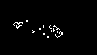
\includegraphics[width=\textwidth]{IMAGES/part2/CGOF_1.png}
        \caption{Iteration 87}
    \end{subfigure}
    \hfill
    \begin{subfigure}{0.35\textwidth}
        \centering
        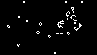
\includegraphics[width=\textwidth]{IMAGES/part2/CGOF_2.png}
        \caption{Iteration 263}
    \end{subfigure}
    \caption{Conway's Game of Life}
    \label{fig:CGOF}
\end{figure}

Programmers, computer scientists, and mathematicians began cataloging all the \href{https://en.wikipedia.org/wiki/Conway's_Game_of_Life#Examples_of_patterns}{patterns they encountered} and constructed remarkably complex machines.

In our case, the rules are defined as follows:
\begin{itemize}  
    \item If there are more than 4 activated cells in the Moore neighborhood, the cell activates. 
    \item Otherwise, the cell deactivates. 
\end{itemize}

I implement the method on a Cartesian grid and then transform it into a triangular mesh, as shown in \autoref{fig:triag_transform}. The maps generated after this transformation improved in quality.

\begin{figure}[H]
	\centering
	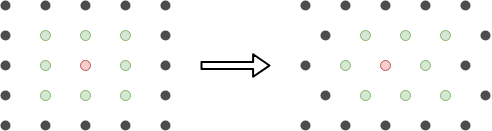
\includegraphics[width=0.6\linewidth]{IMAGES/part2/grid_transform_map_generation.png}
	\caption{Grid transformation}
	\label{fig:triag_transform}
\end{figure}

Using the Marching Squares method, I draw the boundaries between occupied cells (red dots) and unoccupied cells (green dots).

Marching Squares is a technique for generating the contours of a two-dimensional grid, which, in our case, is a triangular mesh. As we traverse the domain, the boundaries are drawn accordingly. \autoref{fig:marching_triag} illustrates all possible states of an element composed of three cells.

\begin{figure}[H]
	\centering
	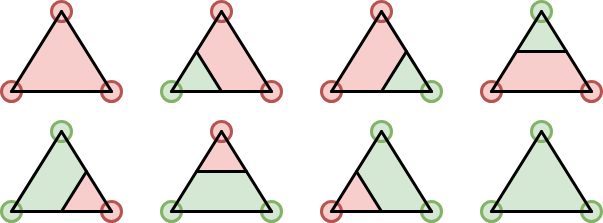
\includegraphics[width=0.6\linewidth]{IMAGES/part2/marching_square_triangle.png}
	\caption{Isolines, possible states of a triangular element}
	\label{fig:marching_triag}
\end{figure}

At the end of both steps—transformation and Marching Squares—we obtain the following schematic representation:

\begin{figure}[H]
	\centering
	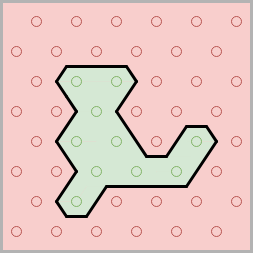
\includegraphics[width=0.3\linewidth]{IMAGES/part2/map_generation_example.png}
	\caption{Exemple scheme of map generated}
	\label{fig:map_gen_scheme}
\end{figure}

In the simulator, maps are generated based on a seed and a random generator. The shape of each map is controlled by three parameters: the step size along the x-axis, the step size along the y-axis, and the overall map size.

This allows for a vast variety of map configurations. \autoref{fig:three_map_example} illustrate some examples.
\begin{figure}[H]
    \centering
    \begin{subfigure}{0.3\textwidth}
        \centering
        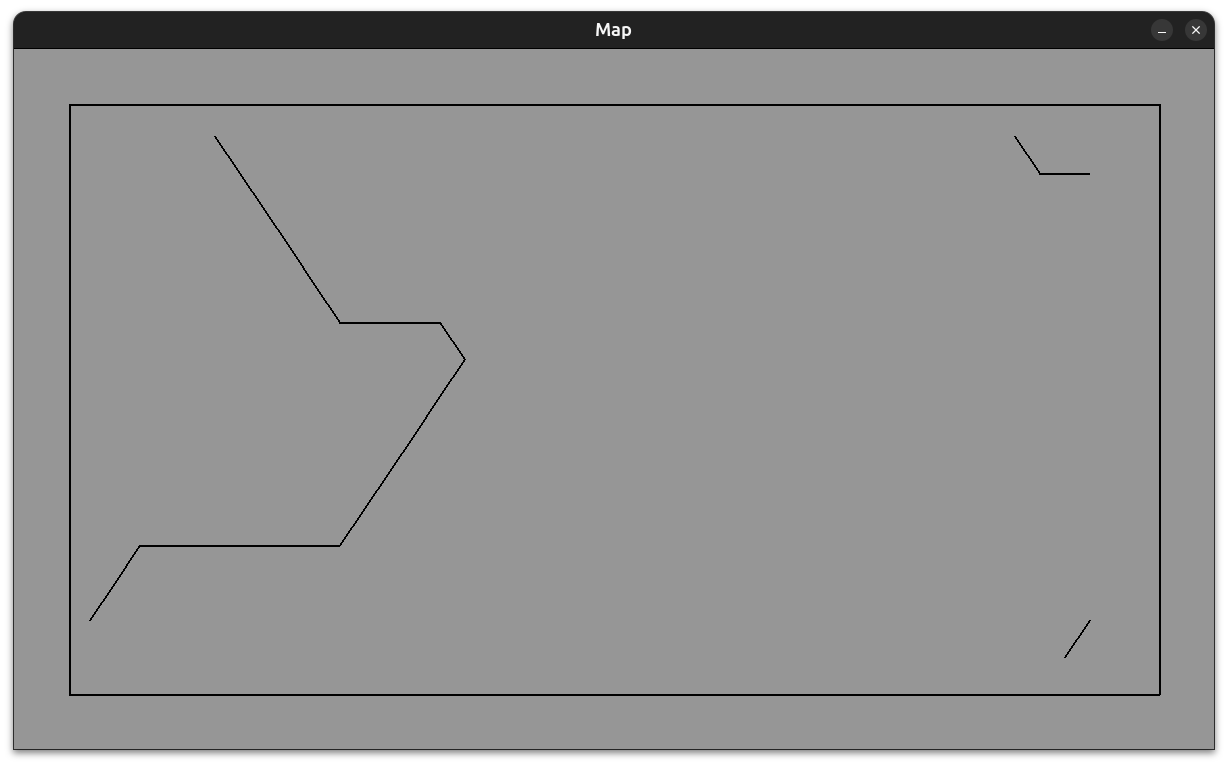
\includegraphics[width=\textwidth]{IMAGES/part2/map_dx100.png}
        \caption{$\delta x = 100$ mu}
    \end{subfigure}
    \hfill
    \begin{subfigure}{0.3\textwidth}
        \centering
        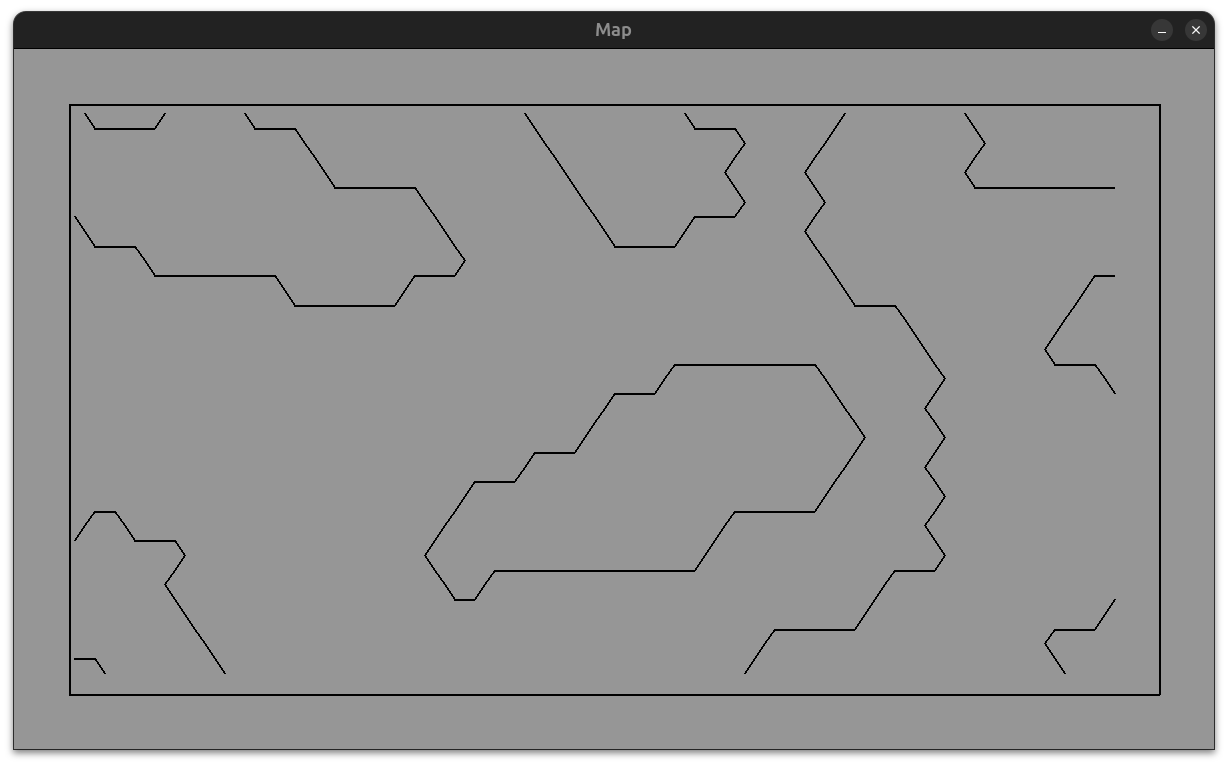
\includegraphics[width=\textwidth]{IMAGES/part2/map_dx40.png}
        \caption{$\delta x = 40$ mu}
    \end{subfigure}
    \hfill
    \begin{subfigure}{0.3\textwidth}
        \centering
        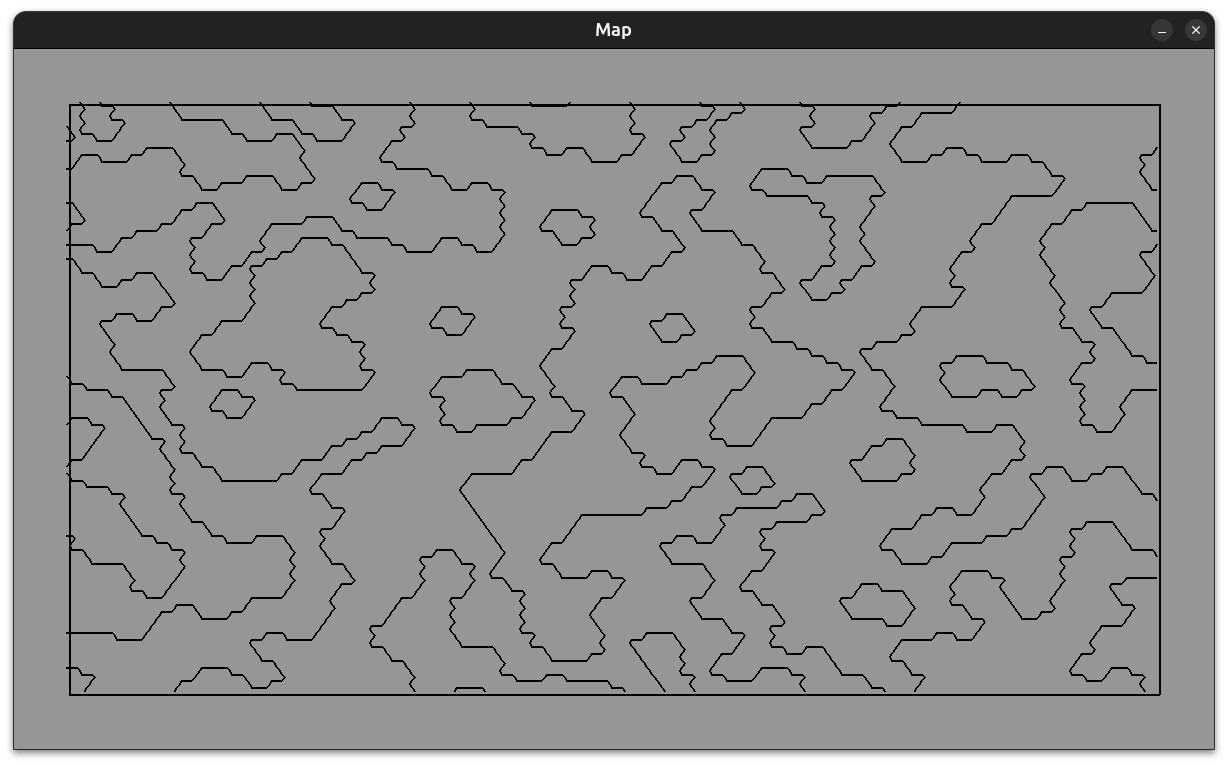
\includegraphics[width=\textwidth]{IMAGES/part2/map_dx10.png}
        \caption{$\delta x = 10$ mu}
    \end{subfigure}
    \caption{Different maps made with equilateral triangles}
    \label{fig:three_map_example}
\end{figure}

\tobedone


\subsection{Robot implementation}


\subsubsection{Sensors}

The robot is equiped with 2 sensors by default, an accelerometer that calculates acceleration in x and y axis and the rotation along z

Simultaneous Localization and Mapping (SLAM) is a key problem in robotics, enabling a robot to determine its position while simultaneously building a map of its environment. Various techniques have been developed to tackle this challenge. For instance, EKF-SLAM uses a Kalman filter to estimate both the localization and the map but faces scalability limitations in large environments. FastSLAM, which relies on a particle filter, enhances scalability by handling world features through multiple hypotheses.  

Graph-based approaches, such as Graph-SLAM, are effective for large-scale optimization problems but require complex data management. Visual SLAM (V-SLAM) leverages cameras to estimate localization and construct maps, whereas LiDAR-based SLAM relies on laser sensors for precise depth measurements, making it particularly useful for outdoor environments. Dynamic SLAM variants manage environments with moving objects by excluding them from map updates.\cite{ding_2024}

In this report, I used LiDAR-based SLAM, 


\end{document}